\documentclass{article}
\usepackage{graphicx}
\usepackage{hyperref}
\usepackage{amsmath}
\usepackage{amssymb}
\usepackage{enumitem}
\usepackage{float}
\usepackage{textcomp}

\renewcommand\labelitemi{---}

\author{Stephen Lee}
\title{Do Tweets Predict Cryptocurrency Price Movements?}
\date{2018}

\begin{document}
	\maketitle
	
	\section{Introduction}
	In 2008, the Bitcoin white paper was published under the pseudonym Satoshi Nakamoto. The paper combined cryptography with a game theoretic incentive structure to provide secure peer-to-peer financial transactions without needing a trusted 3rd party.  Since then, other projects have modified the Bitcoin rules to create new protocols for handling these transactions. Colloquially referred to as ``cryptocurrencies'', these projects have captured the imagination of many. As of May 3, 2018, the three largest cryptocurrencies by market capitalization are Bitcoin, Ether, and Ripple. This paper explores the price movements of these coins in addition to a simple variant of Bitcoin called Litecoin. 
	
	Using trade level data from a European exchange over the dates August 2017 to April 2018, I previously explored the possibility of cointegration and Granger causality - however results so far are inconclusive. Interestingly in the dataset, a massive price bubble appeared from roughly December to February. While a more robust analysis is needed, the data does seem to be seperable into three distinct periods: pre-bubble, bubble, and post-bubble. Blah blah blah about how cointegration seems possible in post-bubble, signifying possible increase in investor awareness. 
	
	Here, I study if Twitter ``tweets'' can be predictive of price movements in the first two weeks of December (i.e. as the bubble was forming). 
	
	\section{Data}
	
	\subsection{Cryptocurrency Transactions}
	Price data comes from the European coin exchange Bitstamp. In it's raw form, the data includes information about each transaction in the history of the exchange, including the unix-timestamp\footnote{The unix-timestamp is given by the number of seconds that have passed since January 1, 1970 at 12:00:00 am GMT}, trade price, and trade quantity. After cleaning, the final series consists of hourly periods ranging from Thursday, August 17, 2017 2:00 pm to Tuesday, April 24, 2018 4:00 am GMT. 
	
	Graphically, the final time series are as follows: 
	\begin{figure}[H]
	\centering
	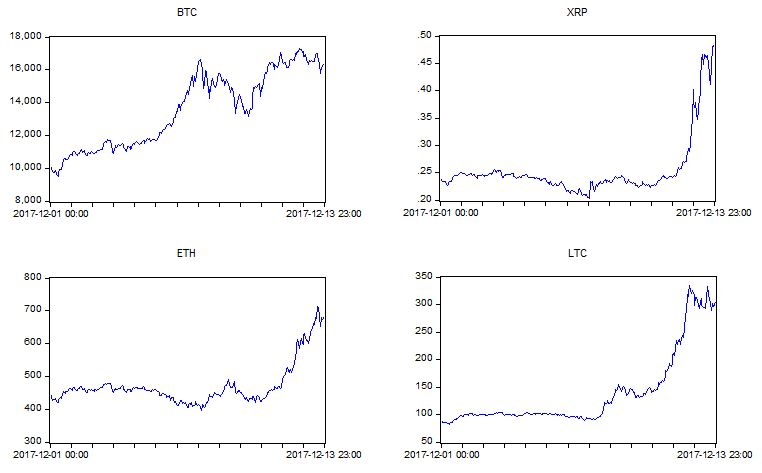
\includegraphics[width = .9\textwidth]{priceSeries.JPG}
	\caption{Time series of Bitcoin, Ether, Ripple, and Litecoin prices every hour.}
	\end{figure}
	
	
	\subsection{Tweets}
	I scraped Twitter's database for every ``tweet'' that mentioned the word Bitcoin from December 1, 2017 00:00, to December 13, 2017 23:00. This required overcoming several challenges: 1) Twitter's official programming interface places strict limits on data accessibility - namely, you are restricted to 150 page requests every 15 minutes, and also you can only access tweets from within the last 7 days; 2) local storage and computational power (i.e. on my laptop) are insufficient for large scraping projects that may need to run for several days; and 3) this raw Twitter data needs to be manipulated and merged with my existing hourly price and volume data in a way that ``best captures'' the tweets. 
	
	Thus, to obtain usable data, I modified an open source project that bypasses the limitations of the official interface.\footnote{Code available here: https://github.com/slee981/TwitterSearch\_API.} Specifically, this project reverse engineers the behavior of the official Twitter access interface by utilizing the same URL and query structure. Additional considerations were made to respect Twitter server's capacity constraints by placing one second between subsequent data requests as per their specs.\footnote{Best practices for Twitter webscraping are described here: https://twitter.com/robots.txt.} Note, however, that due to Twitter's server protection, each web scraper I launched was essentially banned after scraping about a day's worth of Tweets (i.e. about 72,000 tweets). Because of this, a new web scraper and IP address were needed for each day's worth of tweets. Even after trying to run a new scraper repeatedly over the same day and remove duplicates in the data cleaning phase, there are several stretches of missing information - presumably because of Twitters database blocking the requests. 
	
	Next, in order to scrape and store large quantities of data, I created new cloud based computational (Elastic Cloud Compute, EC2) and storage (Relational Database Service, RDS) instances using Amazon Web Services (AWS).
	
	Finally, I re-grouped the data into an hourly timeseries with counts for the total number of tweets, the total retweets, and the total number of favorited tweets. The result was a ``mostly complete'' dataset that consisted of the number of tweets that mentioned the word Bitcoin every hour, corresponding to the same hour as the price and quantity series. As mentioned above, however, there is some missing data. The final series graph is as follows: 
	
	\begin{figure}[H]
	\centering
	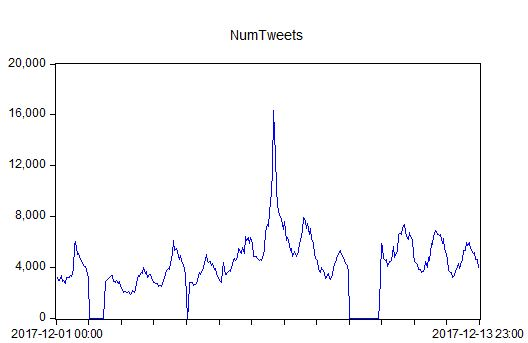
\includegraphics[width = .9\textwidth]{numTweets.JPG}
	\caption{Time series of the number of tweets that mention Bitcoin per hour.}
	\end{figure}
	
	\section{Analysis}
	% PRELIMINARY, NEEDS WORK
	\textbf{The following is based on a first glance analysis of the data.}
	
	First, I regressed the change in BTC price from the previous hour on the number of tweets that mention Bitcoin and find the following results. Note that I add the previous hours change in price to a basic ARIMA(1,1) model based on the initial correlogram of the number of tweets series. 
	\begin{figure}[H]
	\centering
	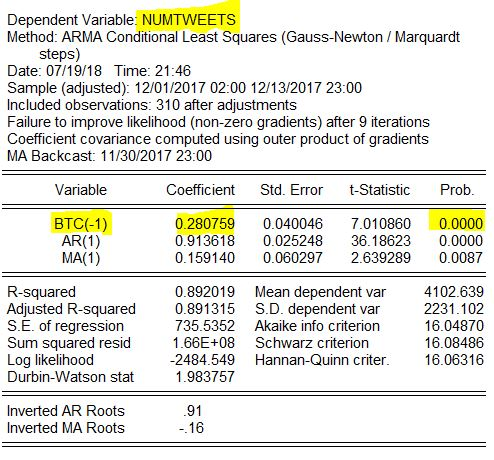
\includegraphics[width = .9\textwidth]{numTweetsRegResults.JPG}
	\end{figure}
	
	This yields the following ACF and PACF and suggests that, with statistical significance, the more the price of Bitcoin changes, the more tweets about it you can expect in the next hour. 
	
	\begin{figure}[H]
	\centering
	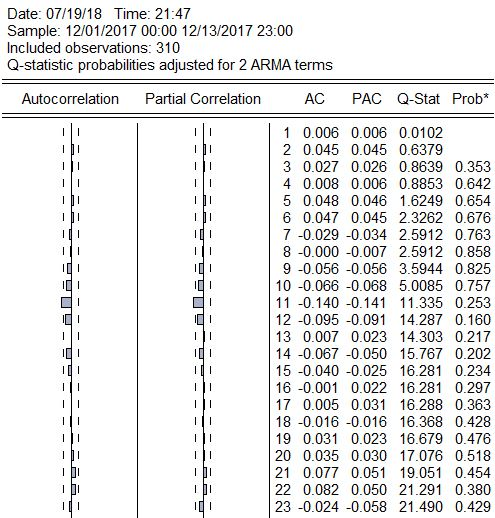
\includegraphics[width = .9\textwidth]{ACF_PACF.JPG}
	\caption{ACF and PACF of residual series from above regression.}
	\end{figure}
	
	
	Similarly, based on the correlogram of the differenced BTC price series (i.e. the change in price), I added the number of tweets that to an AR(3) model and also find significance. This suggests that as more people talk about Bitcoin on twitter, the more the price increases. 
	
	\begin{figure}[H]
	\centering
	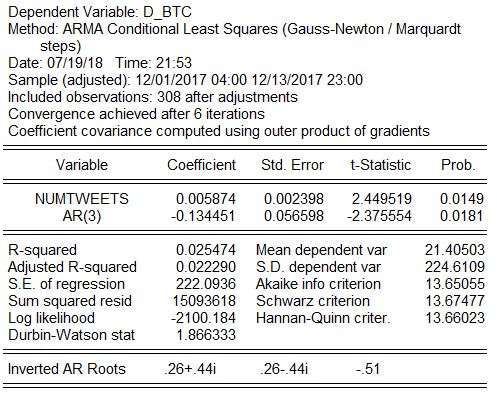
\includegraphics[width = .9\textwidth]{dBtcRegResults.JPG}
	\end{figure}
	
	
	\begin{figure}[H]
	\centering
	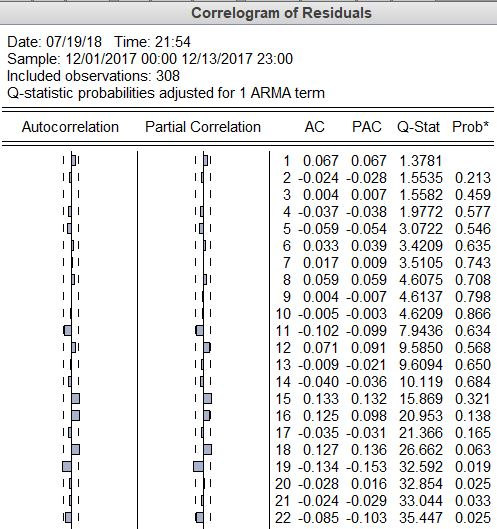
\includegraphics[width = .9\textwidth]{dBtc_ACF.JPG}
	\caption{ACF and PACF of residual series from above regression.}
	\end{figure}
	
	\section{Conclusion}
	
	While this is a VERY preliminary and crude look into the data - the appearance of statistical significance seems worth exploring further. 
	
\end{document}

	
% Itemize
\begin{itemize}
	\item
\end{itemize}

% enumerate
\begin{enumerate}
	\item
\end{enumerate}

% Figures
\begin{figure}[H]
	\centering
	\includegraphics[width = .75\textwidth]{}
	\caption{}
\end{figure}

% Equations
\begin{align}
\begin{split}
\end{split}
\end{align}

% Paragraph
\begin{flushleft}
\end{flushleft}

% Fancy 
\begin{equation}
\mathcal{L}(T,B,\lambda) = 
\end{equation}

% Partials
\begin{align}
\frac{\partial \mathcal{L}}{\partial T} &= 
\frac{\partial \mathcal{L}}{\partial B} &= 
\frac{\partial \mathcal{L}}{\partial \lambda} &= 
\end{align}

%Piecewise
\begin{displaymath}
function = \left\{
\begin{array}{lr}
0 & \quad P\textsubscript{C} < P\textsubscript{P}\\
U\textsubscript{0} & \quad  P\textsubscript{C} > P\textsubscript{P}
\end{array}
\right.
\end{displaymath}
